\newpage
\section{Atividades}

Calcular a resistência equivatente total dos circuitos.

\subsection{ Circuito 1}
Dados:
$R_1 = 1k2\Omega$,
$R_2 = 300\Omega$ e
$R_3 = 120\Omega$.
\begin{figure}[H]
  \centering
  \label{fig:ativ1}
  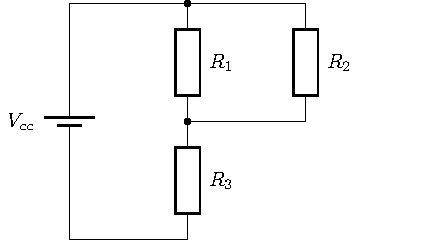
\includegraphics[scale=1.0]{fig-ativ1}
\end{figure}

\subsection{ Circuito 2}
Dados:
$R_1 = 2k7\Omega$,
$R_2 = 24k\Omega$,
$R_3 = 3k3\Omega$ e
$R_4 = 200\Omega$.
\begin{figure}[H]
  \centering
  \label{fig:ativ1}
  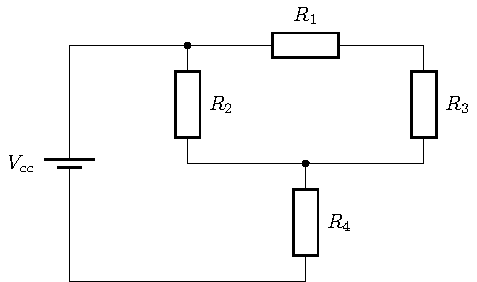
\includegraphics[scale=1.0]{fig-ativ2}
\end{figure}

\subsection{ Circuito 3}
Dados:
$R_1 = 100\Omega$,
$R_2 = 100\Omega$,
$R_3 = 100\Omega$,
$R_4 = 300\Omega$,
$R_5 = 200\Omega$,
$R_6 = 100\Omega$, e
$R_7 = 100\Omega$.
\begin{figure}[H]
  \centering
  \label{fig:ativ1}
  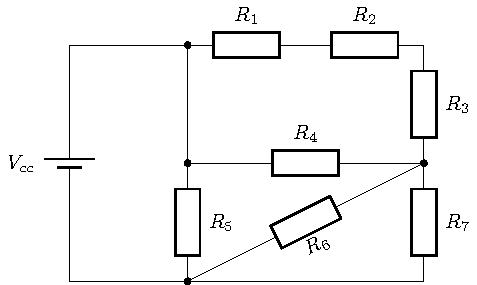
\includegraphics[scale=1.0]{fig-ativ3}
\end{figure}
